\documentclass[12pt]{article}
\usepackage[romanian]{babel}
\usepackage[utf8]{inputenc}
\usepackage[T1]{fontenc}
\usepackage{amsmath, amssymb}
\usepackage{graphicx}
\usepackage{float}
\usepackage{booktabs}
\usepackage{caption}
\usepackage{geometry}
\usepackage{ragged2e}
\usepackage{hyperref}
\usepackage{fancyhdr}
\usepackage{color}
\geometry{a4paper, margin=2.5cm}

\pagestyle{fancy}
\fancyhf{}
\rhead{Grupa 151}
\lhead{Tema 1 de laborator}
\cfoot{\thepage}

\title{\textbf{Tema 1 de laborator}}
\author{Aioanei Florin \and Verzotti Matteo \and Voaides Robert}
\date{}

\begin{document}

\maketitle

\begin{center}
    \textbf{Compararea unor algoritmi de sortare prin comportamentul lor asupra mai multor suite de teste}\\
\end{center}

\vspace{1cm}

\tableofcontents
\newpage

\section{Introducere}

În această lucrare ne propunem să comparăm performanțele mai multor algoritmi de sortare din punct de vedere al complexității teoretice și al performanței practice. Scopul este de a evidenția avantajele și dezavantajele fiecărui algoritm în funcție de dimensiunea și natura datelor de intrare.

\section{Algoritmi analizați}

\begin{itemize}
    \item Quick Sort
    \begin{itemize}
        \item Random Pivot
        \item Median Pivot
        \item Half Pivot
        \item Ternary Quick Sort
    \end{itemize}
    \item Radix Sort
    \begin{itemize}
        \item base 10
        \item base 16
        \item base $2^{16}$
    \end{itemize}
    \item Merge Sort
    \item Intro Sort
    \item Tim Sort
    \item Shell Sort
\end{itemize}

\section{Complexitate teoretică}

\begin{table}[H]
    \centering
    \caption{Tabel comparativ al complexităților algoritmilor analizați}
    \begin{tabular}{lccc}
    \toprule
    \textbf{Algoritm} & \textbf{Best case} & \textbf{Average} & \textbf{Worst Case} \\
    \midrule
    Quick Sort (Random Pivot) & $\mathcal{O}(n \log n)$ & $\mathcal{O}(n \log n)$ & $\mathcal{O}(n^2)$ \\
    Quick Sort (Median Pivot) & $\mathcal{O}(n \log n)$ & $\mathcal{O}(n \log n)$ & $\mathcal{O}(n \log n)$ \\
    Quick Sort (Half Pivot)   & $\mathcal{O}(n \log n)$ & $\mathcal{O}(n \log n)$ & $\mathcal{O}(n^2)$ \\
    Ternary Quick Sort        & $\mathcal{O}(n \log n)$ & $\mathcal{O}(n \log n)$ & $\mathcal{O}(n^2)$ \\
    Radix Sort (base 10)      & $\mathcal{O}(nk)$       & $\mathcal{O}(nk)$       & $\mathcal{O}(nk)$ \\
    Radix Sort (base 16)      & $\mathcal{O}(nk)$       & $\mathcal{O}(nk)$       & $\mathcal{O}(nk)$ \\
    Radix Sort ($2^{16}$)     & $\mathcal{O}(nk)$       & $\mathcal{O}(nk)$       & $\mathcal{O}(nk)$ \\
    Merge Sort                & $\mathcal{O}(n \log n)$ & $\mathcal{O}(n \log n)$ & $\mathcal{O}(n \log n)$ \\
    Intro Sort                & $\mathcal{O}(n \log n)$ & $\mathcal{O}(n \log n)$ & $\mathcal{O}(n \log n)$ \\
    Tim Sort                  & $\mathcal{O}(n)$        & $\mathcal{O}(n \log n)$ & $\mathcal{O}(n \log n)$ \\
    Shell Sort                & $\mathcal{O}(n \log n)$ & $\mathcal{O}(n^{5/4})$  & $\mathcal{O}(n^2)$ \\
    \bottomrule
    \end{tabular}
    \end{table}

\section{Implementare}

\begin{justify}
Toți algoritmii au fost organizați într-un repository GitHub, structurat clar.
Fiecare algoritm de sortare are propriul său header dedicat în folderul include/, iar
implementarea este realizată în fișiere .cpp separate.
\end{justify}


\section{Metodologie experimentală}

Pentru testarea performanțelor, am creat un sistem automatizat de rulare și înregistrare a testelor, organizat în jurul fișierului principal \texttt{main.cpp}. Setările fiecărui test sunt definite într-un fișier de configurare \texttt{test\_config.csv}, unde fiecare linie specifică: \texttt{nameoftest, numberofvalues, maxvalue}. Aceste configurații sunt parcurse și procesate cu ajutorul funcției \texttt{readTestConfigs()}, iar pentru fiecare algoritm de sortare implementat în sistem, se generează un vector aleatoriu corespunzător parametrilor testului.

Toți algoritmii sunt înregistrați într-un map, ce permite selectarea și rularea lor pe baza numelui.

Timpul de execuție pentru fiecare sortare este măsurat cu funcția \texttt{measureTime()}, iar rezultatele sunt salvate în fișierul \texttt{results.csv}, folosind funcția \texttt{logResult()} incluzând: numele testului, algoritmul, dimensiunea vectorului, valoarea maximă, timpul de execuție (în secunde) și dacă vectorul rezultat este sortat corect.

Pentru o testare completă, aplicația poate fi rulată cu comanda \texttt{./main all}, caz în care se rulează toți algoritmii în toate testele definite.

\bigskip

Fiecare algoritm este rulat o singură dată per configurație, iar logica poate fi extinsă ușor pentru repetare multiplă și calculul unei medii. Măsurarea timpului s-a realizat utilizând funcționalități din biblioteca standard \texttt{<chrono>}.

\section{Rezultate experimentale}

\subsection{Numere putine, valori dense}
\begin{figure}[H]
    \centering
    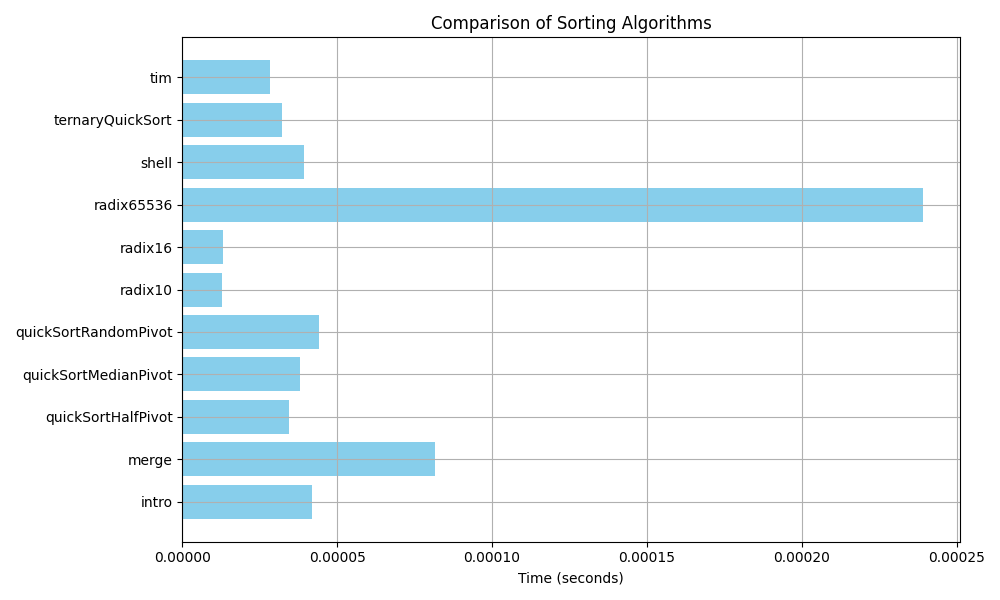
\includegraphics[width=0.8\textwidth]{./img/img_20250417_022149.png} % Replace with your image file path and name
    \caption{Pentru 1000 de numere si valori intre 0 si $10^3$}
\end{figure}
\subsection{Numere putine, valori dispersate}
\begin{figure}[H]
    \centering
    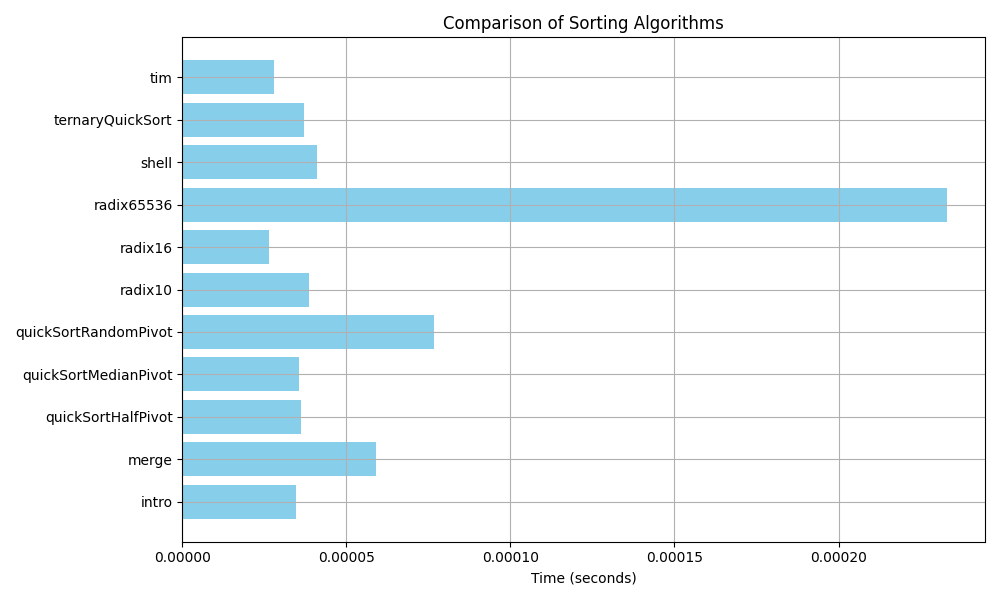
\includegraphics[width=0.8\textwidth]{./img/img_20250417_022311.png} % Replace with your image file path and name
    \caption{Pentru 1000 de numere si valori intre 0 si $10^9$}
\end{figure}
\subsection{Numere multe, valori dense}
\begin{figure}[H]
    \centering
    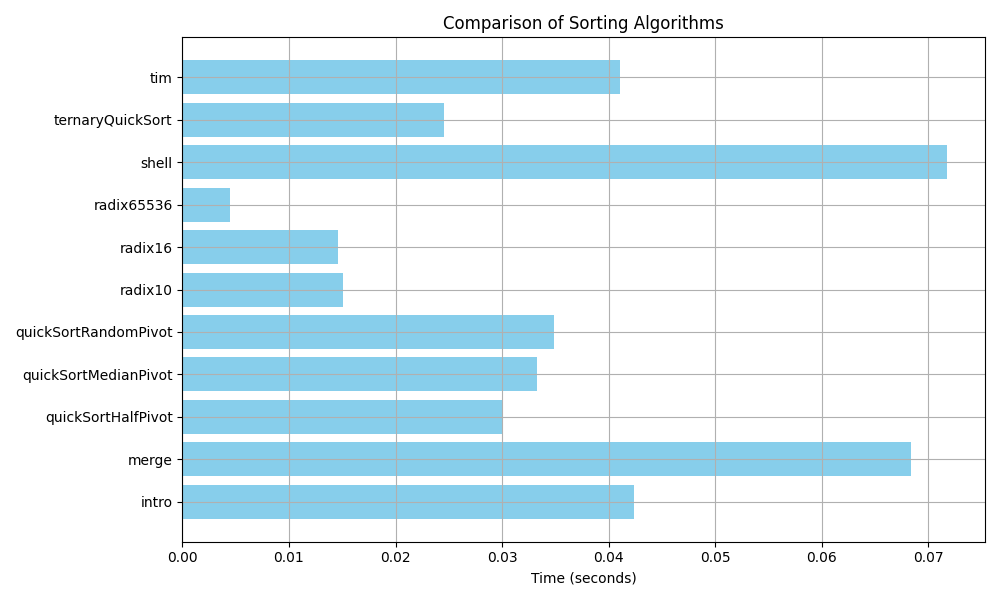
\includegraphics[width=0.8\textwidth]{./img/img_20250417_022351.png} % Replace with your image file path and name
    \caption{Pentru $10^6$ numere si valori intre 0 si $10^3$}
\end{figure}
\subsection{Numere multe, valori dispersate}
\begin{figure}[H]
    \centering
    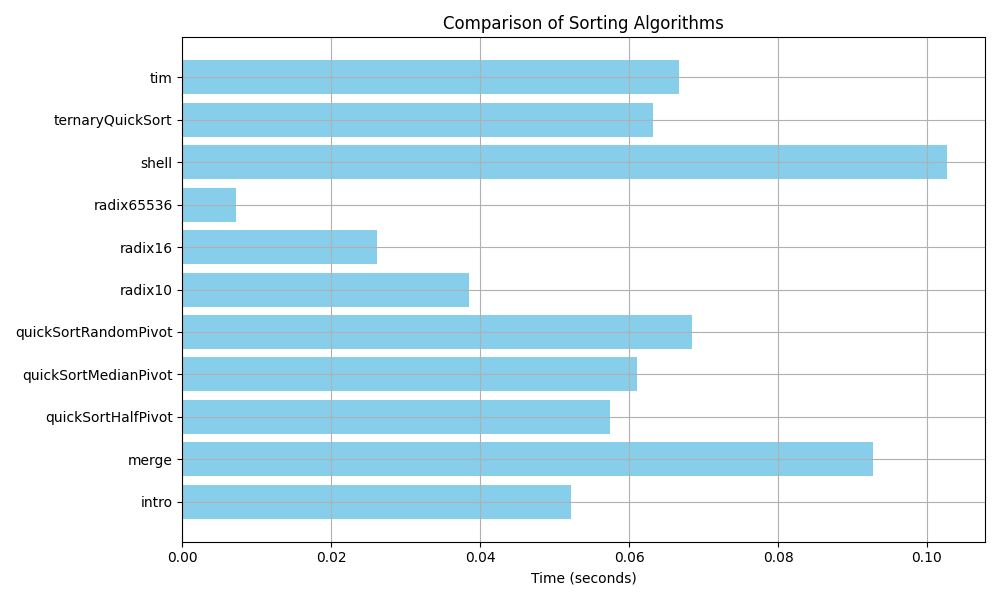
\includegraphics[width=0.8\textwidth]{./img/img_20250417_022431.png} % Replace with your image file path and name
    \caption{Pentru $10^6$ numere si valori intre 0 si $10^9$}
\end{figure}
\subsection{Numere mai multe, valori dense}
\begin{figure}[H]
    \centering
    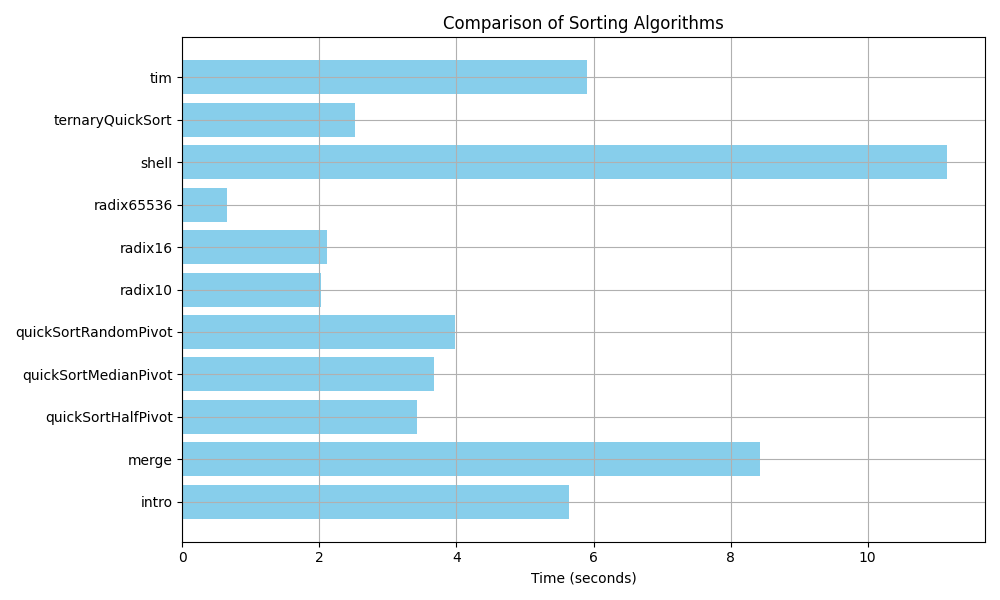
\includegraphics[width=0.8\textwidth]{./img/img_20250417_022629.png} % Replace with your image file path and name
    \caption{Pentru $10^8$ numere si valori intre 0 si $10^3$}
\end{figure}
\subsection{Numere mai multe, valori dispersate}
\begin{figure}[H]
    \centering
    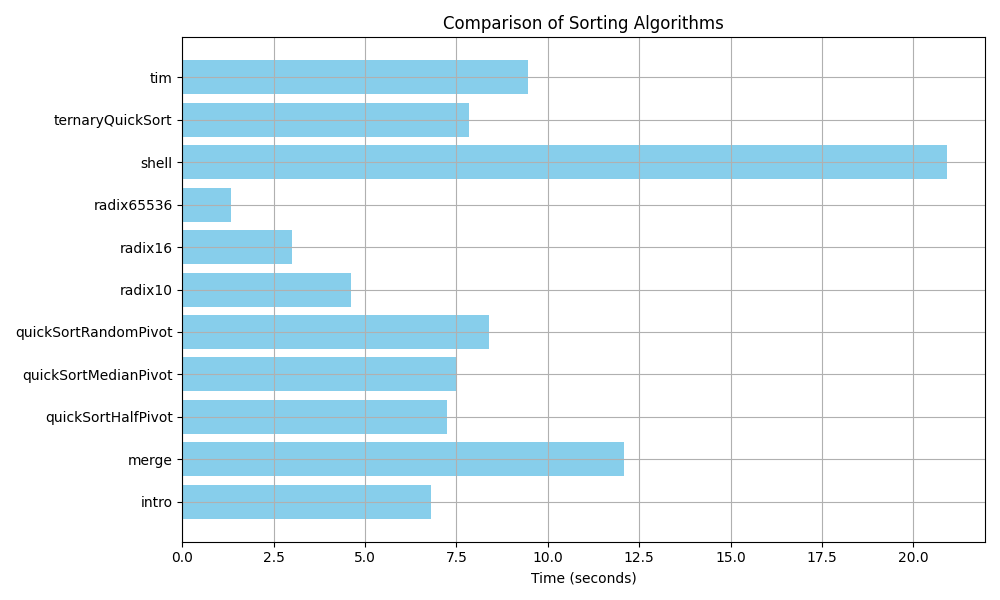
\includegraphics[width=0.8\textwidth]{./img/img_20250417_022859.png} % Replace with your image file path and name
    \caption{Pentru $10^8$ numere si valori intre 0 si $10^9$}
\end{figure}
\subsection{Numere mai multe, o singura valoare}
\begin{figure}[H]
    \centering
    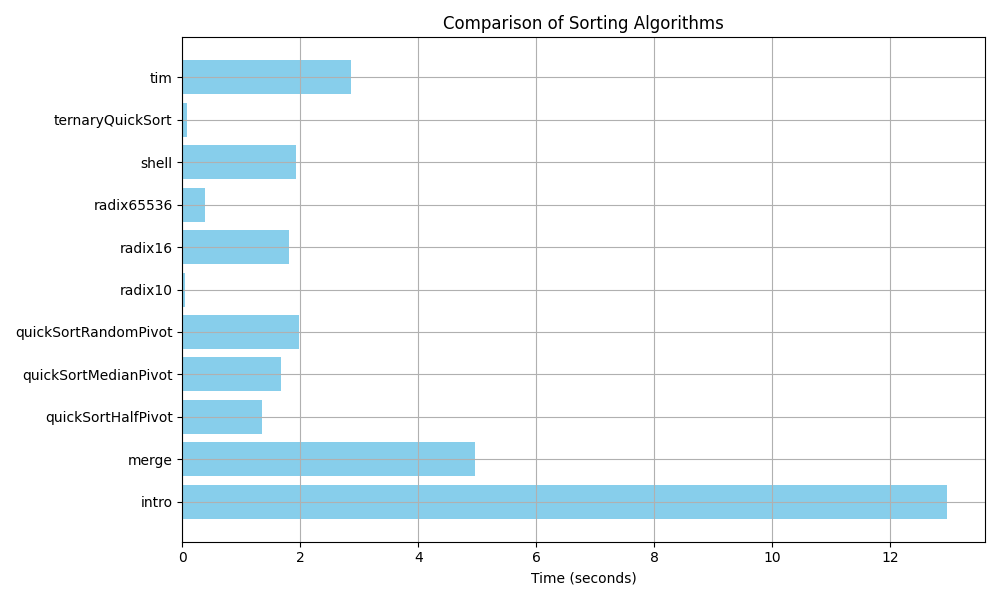
\includegraphics[width=0.8\textwidth]{./img/img_20250417_023613.png} % Replace with your image file path and name
    \caption{Pentru $10^8$ numere egale cu 0}
\end{figure}
\subsection{Numere mai multe, 2 valori}
\begin{figure}[H]
    \centering
    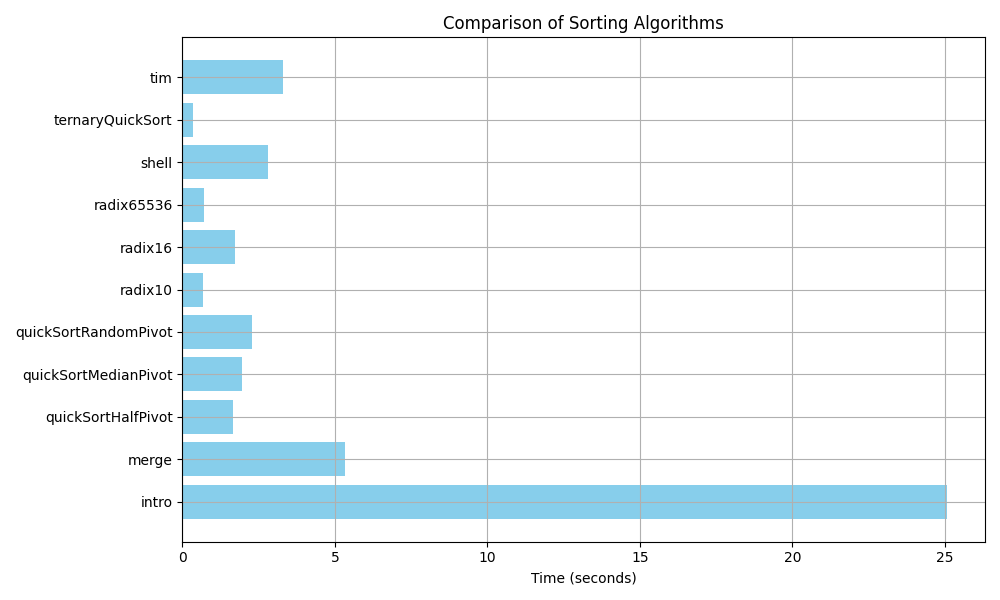
\includegraphics[width=0.8\textwidth]{./img/img_20250417_023757.png} % Replace with your image file path and name
    \caption{Pentru $10^8$ numere egale cu 0 sau 1}
\end{figure}
\subsection{Numere mai multe, 11 valori}
\begin{figure}[H]
    \centering
    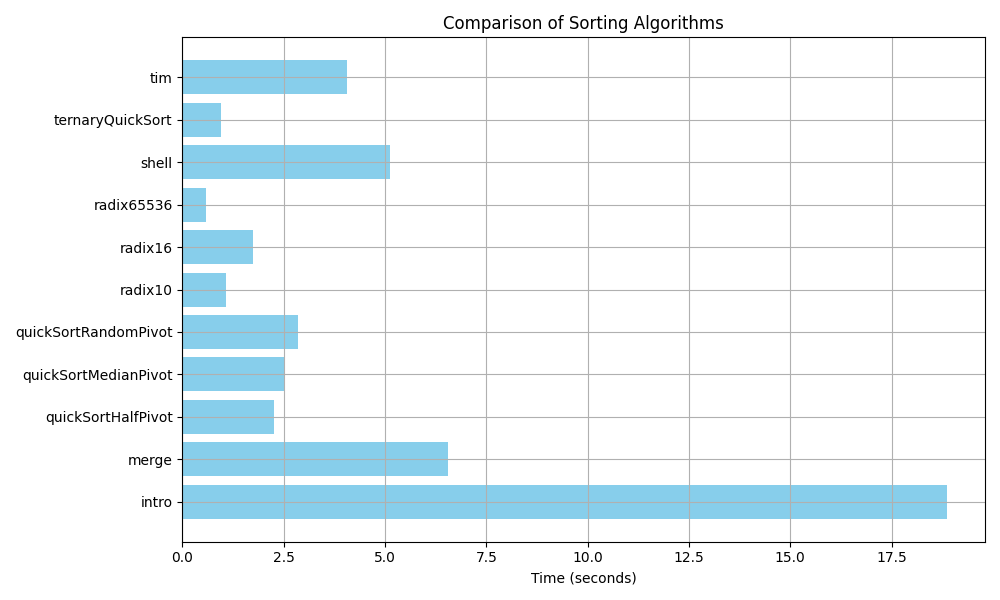
\includegraphics[width=0.8\textwidth]{./img/img_20250417_023946.png} % Replace with your image file path and name
    \caption{Pentru $10^8$ numere egale cu numere de la 0 la 10}
\end{figure}

\section{Concluzii}

\begin{justify}
        Analiza comparativă a evidențiat diferențe semnificative între algoritmii de sortare, atât în ceea ce privește complexitatea teoretică, cât și comportamentul practic în diverse scenarii. Quick Sort, în variantele sale, a demonstrat performanțe bune în medie, însă sensibilitatea la alegerea pivotului poate conduce la cazuri nefavorabile, în special pentru date deja parțial sortate sau cu distribuții neuniforme.

Radix Sort s-a remarcat ca fiind extrem de eficient pentru date numerice cu valori mici și dense, mai ales în variantele cu baze mari, dar depinde de specificul datelor și nu este o soluție universală. Merge Sort și Tim Sort s-au dovedit a fi opțiuni robuste și stabile, potrivite pentru sortări sigure și consistente indiferent de structura datelor. Tim Sort, în particular, a excelat în cazurile în care datele conțineau subsecvențe deja sortate, beneficiind de optimizările sale adaptative.

Shell Sort a avut performanțe intermediare, dar inconsistente, fiind mai puțin recomandat pentru seturi de date mari. În schimb, algoritmi hibrizi precum Intro Sort combină eficiența și siguranța, fiind potriviți în aplicații generale unde este nevoie de control asupra timpului de execuție și de evitare a celor mai nefavorabile cazuri.

În concluzie, alegerea algoritmului de sortare trebuie realizată în funcție de natura și dimensiunea datelor de intrare, precum și de cerințele specifice ale aplicației: timp de execuție, stabilitate, sau complexitate în implementare. \end{justify}

\end{document}
